%Skriv kort introduktion til hvert bilag

% For .TEX:
%\input{FILSTI/FILNAVN}

% For .PDF:
%\chapter{NAVN}
%\label{app:LABEL}
%\includepdf[pages={-}]{FILSTI/FILNAVN}
\chapter{ISO226 Data}
\label{app:ISO226Raadata}
%
Lydtryksniveauer til de otte phon-kurver i det opgivne frekvensområde, svarende til hvad der er opgivet i \textcite[ss. 6-7]{STD:ISO226}.
%
\begin{table}[H]
\centering
\resizebox{\textwidth}{!}{%
\begin{tabular}{|r|r|r|r|r|r|r|r|r|}
\hline
Frekvens{[}Hz{]} & \multicolumn{1}{l|}{20phon} & \multicolumn{1}{l|}{30phon} & \multicolumn{1}{l|}{40phon} & \multicolumn{1}{l|}{50phon} & \multicolumn{1}{l|}{60phon} & \multicolumn{1}{l|}{70phon} & \multicolumn{1}{l|}{80phon} & \multicolumn{1}{l|}{90phon} \\ \hline
20 & 89.6 & 94.8 & 99.9 & 104.7 & 109.5 & 114.3 & 119 & 123.7 \\ \hline
25 & 82.7 & 88.5 & 93.9 & 99.1 & 104.2 & 109.2 & 114.2 & 119.2 \\ \hline
31.5 & 76 & 82.4 & 88.2 & 93.7 & 99.1 & 104.4 & 109.6 & 114.9 \\ \hline
40 & 69.9 & 76.5 & 82.6 & 88.5 & 94.2 & 99.8 & 105.3 & 110.9 \\ \hline
50 & 64 & 71.3 & 77.8 & 84 & 90 & 95.9 & 101.7 & 107.5 \\ \hline
63 & 58.6 & 66.2 & 73.1 & 79.6 & 85.9 & 92.2 & 98.4 & 104.5 \\ \hline
80 & 53.2 & 61.2 & 68.5 & 75.4 & 82.1 & 88.6 & 95.2 & 101.7 \\ \hline
100 & 48.4 & 56.8 & 64.4 & 71.6 & 78.7 & 85.6 & 92.5 & 99.3 \\ \hline
125 & 43.9 & 52.6 & 60.6 & 68.2 & 75.6 & 82.9 & 90.1 & 97.3 \\ \hline
160 & 39.4 & 48.4 & 56.7 & 64.7 & 72.5 & 80.2 & 87.8 & 95.4 \\ \hline
200 & 35.5 & 44.8 & 53.4 & 61.7 & 69.9 & 77.9 & 85.9 & 93.9 \\ \hline
250 & 32 & 41.5 & 50.4 & 59 & 67.5 & 75.9 & 84.3 & 92.6 \\ \hline
315 & 28.7 & 38.4 & 47.6 & 56.5 & 65.4 & 74.2 & 82.9 & 91.6 \\ \hline
400 & 25.7 & 35.5 & 45 & 54.3 & 63.5 & 72.6 & 81.7 & 90.8 \\ \hline
500 & 23.4 & 33.4 & 43.1 & 52.6 & 62.1 & 71.5 & 80.9 & 90.2 \\ \hline
630 & 21.5 & 31.5 & 41.3 & 51.1 & 60.8 & 70.5 & 80.2 & 89.8 \\ \hline
800 & 20.1 & 30.1 & 40.1 & 50 & 59.9 & 69.8 & 79.7 & 89.6 \\ \hline
1000 & 20 & 30 & 40 & 50 & 60 & 70 & 80 & 90 \\ \hline
1250 & 21.5 & 31.6 & 41.8 & 52 & 62.2 & 72.3 & 82.5 & 92.6 \\ \hline
1600 & 21.4 & 32 & 42.5 & 52.9 & 63.2 & 73.5 & 83.7 & 94 \\ \hline
2000 & 18.2 & 28.8 & 39.2 & 49.6 & 60 & 70.3 & 80.6 & 90.9 \\ \hline
2500 & 15.4 & 26 & 36.5 & 46.9 & 57.3 & 67.6 & 77.9 & 88.2 \\ \hline
3150 & 14.3 & 25 & 35.6 & 46.1 & 56.4 & 66.8 & 77.1 & 87.4 \\ \hline
4000 & 15.1 & 26 & 36.6 & 47.1 & 57.6 & 68 & 78.3 & 88.7 \\ \hline
5000 & 18.6 & 29.4 & 40 & 50.5 & 60.9 & 71.3 & 81.6 &  \\ \hline
6300 & 25 & 35.5 & 45.8 & 56.1 & 66.4 & 76.6 & 86.8 &  \\ \hline
8000 & 31.5 & 41.7 & 51.8 & 61.8 & 71.7 & 81.5 & 91.4 &  \\ \hline
10000 & 34.4 & 44.6 & 54.3 & 63.8 & 73.2 & 82.5 & 91.7 &  \\ \hline
12500 & 33 & 42.5 & 51.5 & 60.1 & 68.6 & 77 & 85.4 &  \\ \hline
\end{tabular}%
}
\caption{Lydtryksniveauerne til de specifikke phon-kurver er angivet i dB SPL.}
\label{tab:ISO226Raadata}
\end{table}
\chapter{ISO226 Difference}
\label{app:ISO226Difference}
%
I \autoref{tab:ISO226Difference} fremgår den udregnede difference mellem datapunkterne tilhørende hver phon-kurve og datapunkterne tilhørende referencen ved 80 phon og ved 1000Hz. Ydermere adderes der en forskydningsfaktor, som er den numeriske difference mellem den specifikke phon-kurve og referencen. 
%
\begin{table}[H]
\centering
\resizebox{\textwidth}{!}{%
\begin{tabular}{|r|r|r|r|r|r|r|r|r|}
\hline
\multicolumn{1}{|l|}{Frekvens{[}Hz{]}} & \multicolumn{1}{l|}{20phon} & \multicolumn{1}{l|}{30phon} & \multicolumn{1}{l|}{40phon} & \multicolumn{1}{l|}{50phon} & \multicolumn{1}{l|}{60phon} & \multicolumn{1}{l|}{70phon} & \multicolumn{1}{l|}{80 phon} & \multicolumn{1}{l|}{90phon} \\ \hline
20 & 30.6 & 25.8 & 20.9 & 15.7 & 10.5 & 5.3 & 0 & -5.3 \\ \hline
25 & 28.5 & 24.3 & 19.7 & 14.9 & 10 & 5 & 0 & -5 \\ \hline
31.5 & 26.4 & 22.8 & 18.6 & 14.1 & 9.5 & 4.8 & 0 & -4.7 \\ \hline
40 & 24.6 & 21.2 & 17.3 & 13.2 & 8.9 & 4.5 & 0 & -4.4 \\ \hline
50 & 22.3 & 19.6 & 16.1 & 12.3 & 8.3 & 4.2 & 0 & -4.2 \\ \hline
63 & 20.2 & 17.8 & 14.7 & 11.2 & 7.5 & 3.8 & 0 & -3.9 \\ \hline
80 & 18 & 16 & 13.3 & 10.2 & 6.9 & 3.4 & 0 & -3.5 \\ \hline
100 & 15.9 & 14.3 & 11.9 & 9.1 & 6.2 & 3.1 & 0 & -3.2 \\ \hline
125 & 13.8 & 12.5 & 10.5 & 8.1 & 5.5 & 2.8 & 0 & -2.8 \\ \hline
160 & 11.6 & 10.6 & 8.9 & 6.9 & 4.7 & 2.4 & 0 & -2.4 \\ \hline
200 & 9.6 & 8.9 & 7.5 & 5.8 & 4 & 2 & 0 & -2 \\ \hline
250 & 7.7 & 7.2 & 6.1 & 4.7 & 3.2 & 1.6 & 0 & -1.7 \\ \hline
315 & 5.8 & 5.5 & 4.7 & 3.6 & 2.5 & 1.3 & 0 & -1.3 \\ \hline
400 & 4 & 3.8 & 3.3 & 2.6 & 1.8 & 0.9 & 0 & -0.9 \\ \hline
500 & 2.5 & 2.5 & 2.2 & 1.7 & 1.2 & 0.6 & 0 & -0.7 \\ \hline
630 & 1.3 & 1.3 & 1.1 & 0.9 & 0.6 & 0.3 & 0 & -0.4 \\ \hline
800 & 0.4 & 0.4 & 0.4 & 0.3 & 0.2 & 0.1 & 0 & -0.1 \\ \hline
1000 & 0 & 0 & 0 & 0 & 0 & 0 & 0 & 0 \\ \hline
1250 & -1 & -0.9 & -0.7 & -0.5 & -0.3 & -0.2 & 0 & 0.1 \\ \hline
1600 & -2.3 & -1.7 & -1.2 & -0.8 & -0.5 & -0.2 & 0 & 0.3 \\ \hline
2000 & -2.4 & -1.8 & -1.4 & -1 & -0.6 & -0.3 & 0 & 0.3 \\ \hline
2500 & -2.5 & -1.9 & -1.4 & -1 & -0.6 & -0.3 & 0 & 0.3 \\ \hline
3150 & -2.8 & -2.1 & -1.5 & -1 & -0.7 & -0.3 & 0 & 0.3 \\ \hline
4000 & -3.2 & -2.3 & -1.7 & -1.2 & -0.7 & -0.3 & 0 & 0.4 \\ \hline
5000 & -3 & -2.2 & -1.6 & -1.1 & -0.7 & -0.3 & 0 &  \\ \hline
6300 & -1.8 & -1.3 & -1 & -0.7 & -0.4 & -0.2 & 0 &  \\ \hline
8000 & 0.1 & 0.3 & 0.4 & 0.4 & 0.3 & 0.1 & 0 &  \\ \hline
10000 & 2.7 & 2.9 & 2.6 & 2.1 & 1.5 & 0.8 & 0 &  \\ \hline
12500 & 7.6 & 7.1 & 6.1 & 4.7 & 3.2 & 1.6 & 0 &  \\ \hline
\end{tabular}%
}
\caption{Datasæt der bygger på differencen mellem de individuelle phon-kurver og referencen på 80 phon og ved 1000Hz. Differencerne er angivet i dB SPL.}
\label{tab:ISO226Difference}
\end{table}
\chapter{Udledning af overføringsfunktioner}
\label{app:Overfoeringsfunktion}
%
Med udgangspunkt i to RC-led udledes følgende overføringsfunktion:
%
\begin{equation}
        \frac{V_{out}}{V_{in}} = -\frac{R_F'||\left(R_2+\frac{1}{s*C_2}\right)}{R_i}
\end{equation}
%
\begin{equation}
        = - \frac{R_F'+\left(R_2+\frac{1}{s*C_2}\right)}{R_i*\left(s*C_2*R_F'*\left(R_2+\frac{1}{s*C_2}\right)\right)}
\end{equation}
%
Udtrykket reduceres ved at multiplicere $s*C_2$ i tæller og nævner:
%
\begin{equation}
        = - \frac{R_F'+\left(s*C_2*R_2+1\right)}{R_i*\left(s*C_2*R_F'+\left(s*C_2*R_2+1\right)\right)}
\end{equation}
%
Så kan $-R_F'$ og $R_i$ trækkes ud:
%
\begin{equation}
        = -\frac{R_F'}{R_i}*\frac{s*C_2*R_2+1}{s*C_2*\left(R_F'+R_2\right)+1}
\end{equation}
% 
Hvis $C_2$ $\longrightarrow$ $\infty$ vil det resultere i en DC-forstærkning på:
%
\begin{equation}
        \frac{V_{out}}{V_{in}} = -\frac{R_F'}{R_i}*1
\end{equation}
%
Hvis det ikke er tilfældet, og $C_2$ ikke går mod $\infty$ så vil der være et pol/nulpunkt par, hvor nulpunktet udledes ved:
%
\begin{equation}
        \omega_z = \frac{1}{R*C} 
\end{equation}
%
\begin{equation}
         s*C_2*R_2 = \frac{s}{\omega_z}
\end{equation}
%
Og polen ved:
%
\begin{equation}
        \omega_p = \frac{1}{C_2\left(R_F'+R_2\right)}
\end{equation}
%
\begin{equation}
        s*C_2\left(R_F'+R_2\right) = \frac{s}{\omega_p}
\end{equation}
%
Derfra udledes den endelige overføringsfunktion:
%
\begin{equation}
        -\frac{R_F'}{R_i}*\frac{\left(\frac{s}{\omega_z}+1\right)}{\left(\frac{s}{\omega_p}+1\right)}
\end{equation}
%
Hvis $f = \infty$ så bliver impedansen af tilbagekoblingen, parallelforbindelsen mellem $R_2||R_F'$, hvorfra det fåes:
%
\begin{equation}
        \frac{R_2||R_F'}{R_i}
\end{equation}
% 
Med udgangspunkt i tre RC-led udledes følgende overføringsfunktion:
%
\begin{equation}
        \frac{V_{out}}{V_{in}} = -\frac{R_F''||\left(R_3+\frac{1}{s*C_3}\right)}{R_i}
\end{equation}
%
\begin{equation}
        = - \frac{R_F''+\left(R_3+\frac{1}{s*C_3}\right)}{R_i*\left(s*C_3*R_F''*\left(R_3+\frac{1}{s*C_3}\right)\right)}
\end{equation}
%
Udtrykket reduceres ved at multiplicere $s*C_3$ i tæller og nævner:
%
\begin{equation}
        = - \frac{R_F''+\left(s*C_3*R_3+1\right)}{R_i*\left(s*C_3*R_F''+\left(s*C_3*R_3+1\right)\right)}
\end{equation}
%
Så kan $-R_F''$ og $R_i$ trækkes ud:
%
\begin{equation}
        = -\frac{R_F''}{R_i}*\frac{s*C_3*R_3+1}{s*C_3*\left(R_F''+R_3\right)+1}
\end{equation}
% 
Hvis $C_3$ $\longrightarrow$ $\infty$ vil det resultere i en DC-forstærkning på:
%
\begin{equation}
        \frac{V_{out}}{V_{in}} = -\frac{R_F''}{R_i}*1
\end{equation}
%
Hvis det ikke er tilfældet, og $C_3$ ikke går mod $\infty$ så vil der være et pol/nulpunkt par, hvor nulpunktet udledes ved:
%
\begin{equation}
        \omega_z = \frac{1}{R*C} 
\end{equation}
%
\begin{equation}
         s*C_3*R_3 = \frac{s}{\omega_z}
\end{equation}
%
Og polen ved:
%
\begin{equation}
        \omega_p = \frac{1}{C_3\left(R_F''+R_3\right)}
\end{equation}
%
\begin{equation}
        s*C_3\left(R_F''+R_3\right) = \frac{s}{\omega_p}
\end{equation}
%
Derfra udledes den endelige overføringsfunktion:
%
\begin{equation}
        -\frac{R_F''}{R_i}*\frac{\left(\frac{s}{\omega_z}+1\right)}{\left(\frac{s}{\omega_p}+1\right)}
\end{equation}
%
Hvis $f = \infty$ så bliver impedansen af tilbagekoblingen, parallelforbindelsen mellem $R_3||R_F''$, hvorfra det fåes:
%
\begin{equation}
        \frac{R_3||R_F''}{R_i}
\end{equation}
% 


%
\chapter{Beregninger af RC-led}
Indeholder beregninger for filtre med 1, 2, 3, 4 og 8 RC-led.
\label{app:Beregninger af RC-led}
\includepdf[pages={-}]{Content/Bilag/BeregningerRC-led}
%
\chapter{Beregninger for 5.24 dB forstærkning}
Indeholder beregninger for filtre som giver 5.24 dB forstærkning.
\label{app:3RCledGain5.24}
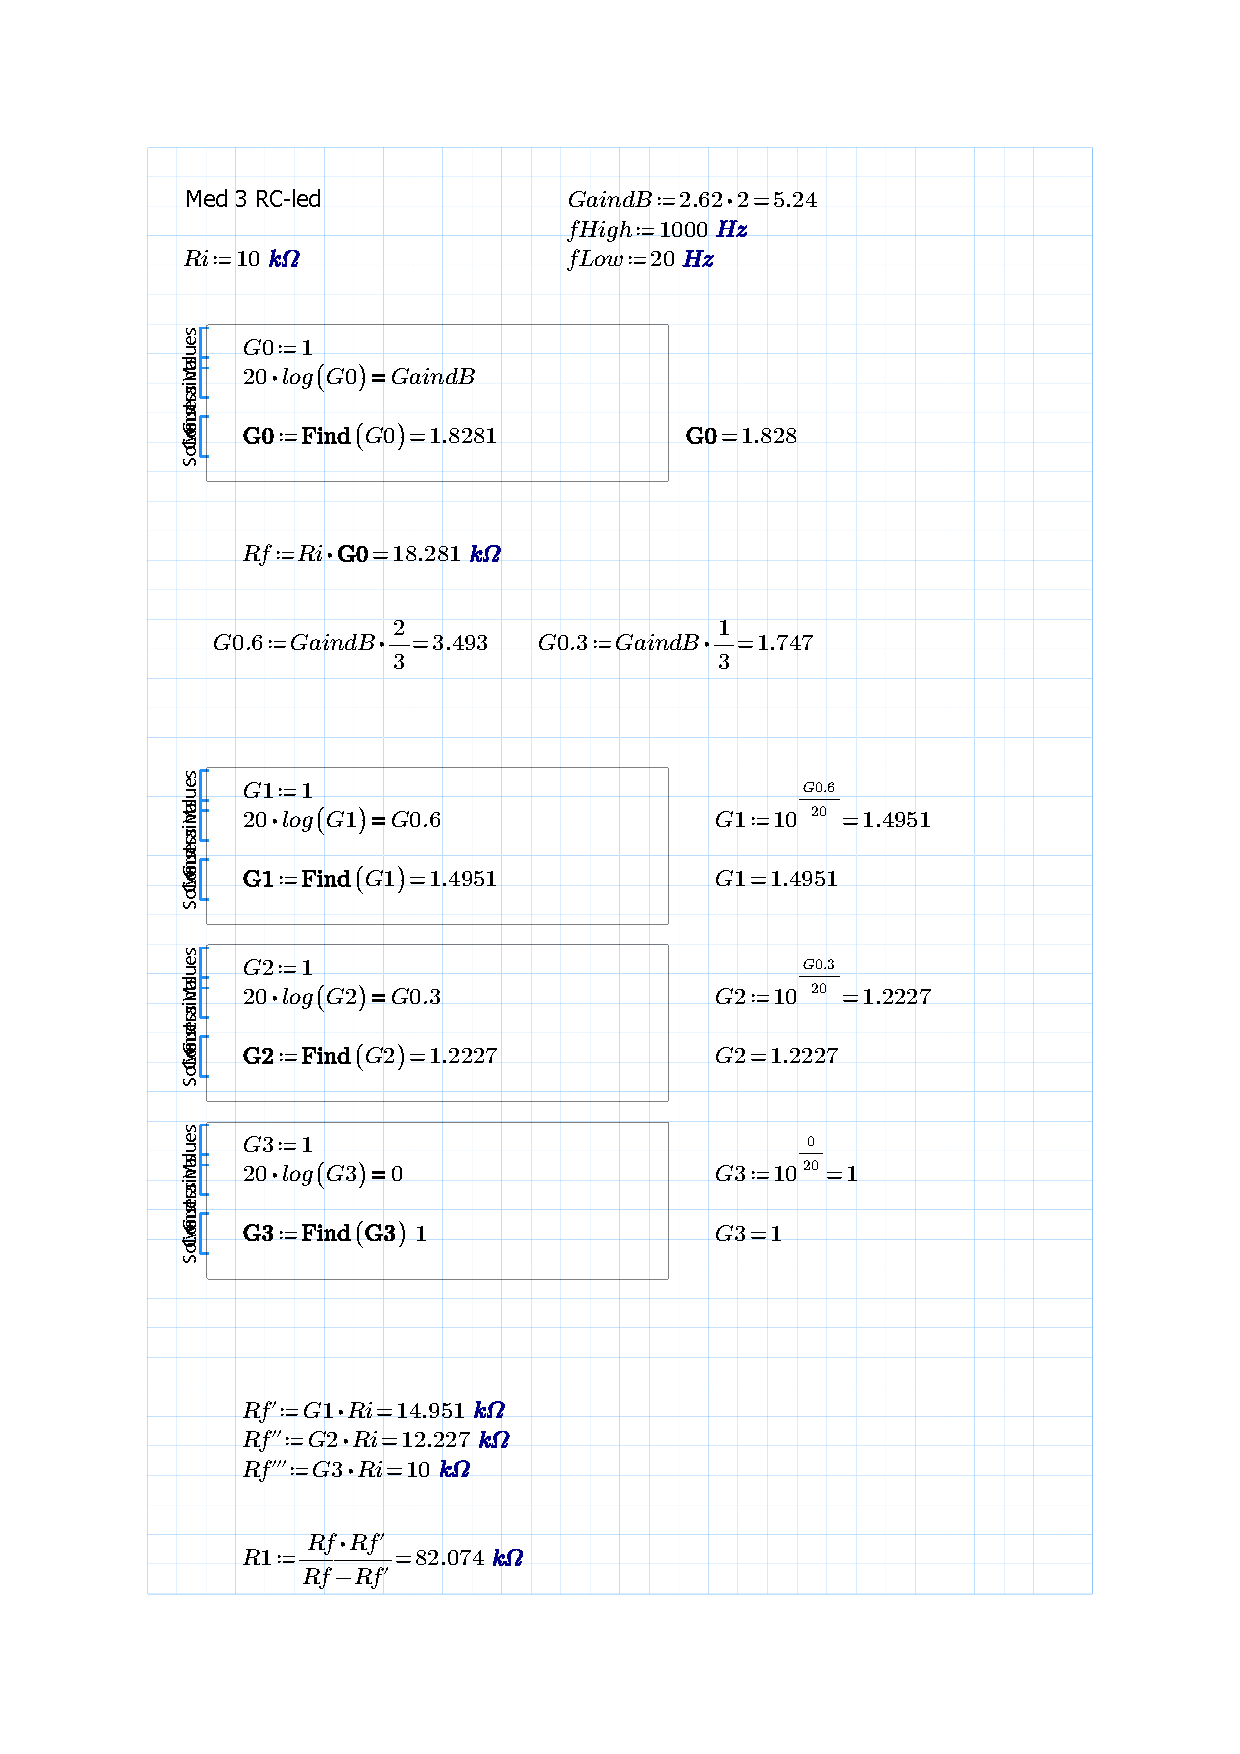
\includepdf[pages={-}]{Content/Bilag/3RCledGain5_24.pdf}
%
\chapter{Beregninger for 10.48 dB forstærkning}
Indeholder beregninger for filtre som giver 10.48 dB forstærkning.
\label{app:3RCledGain10.48}
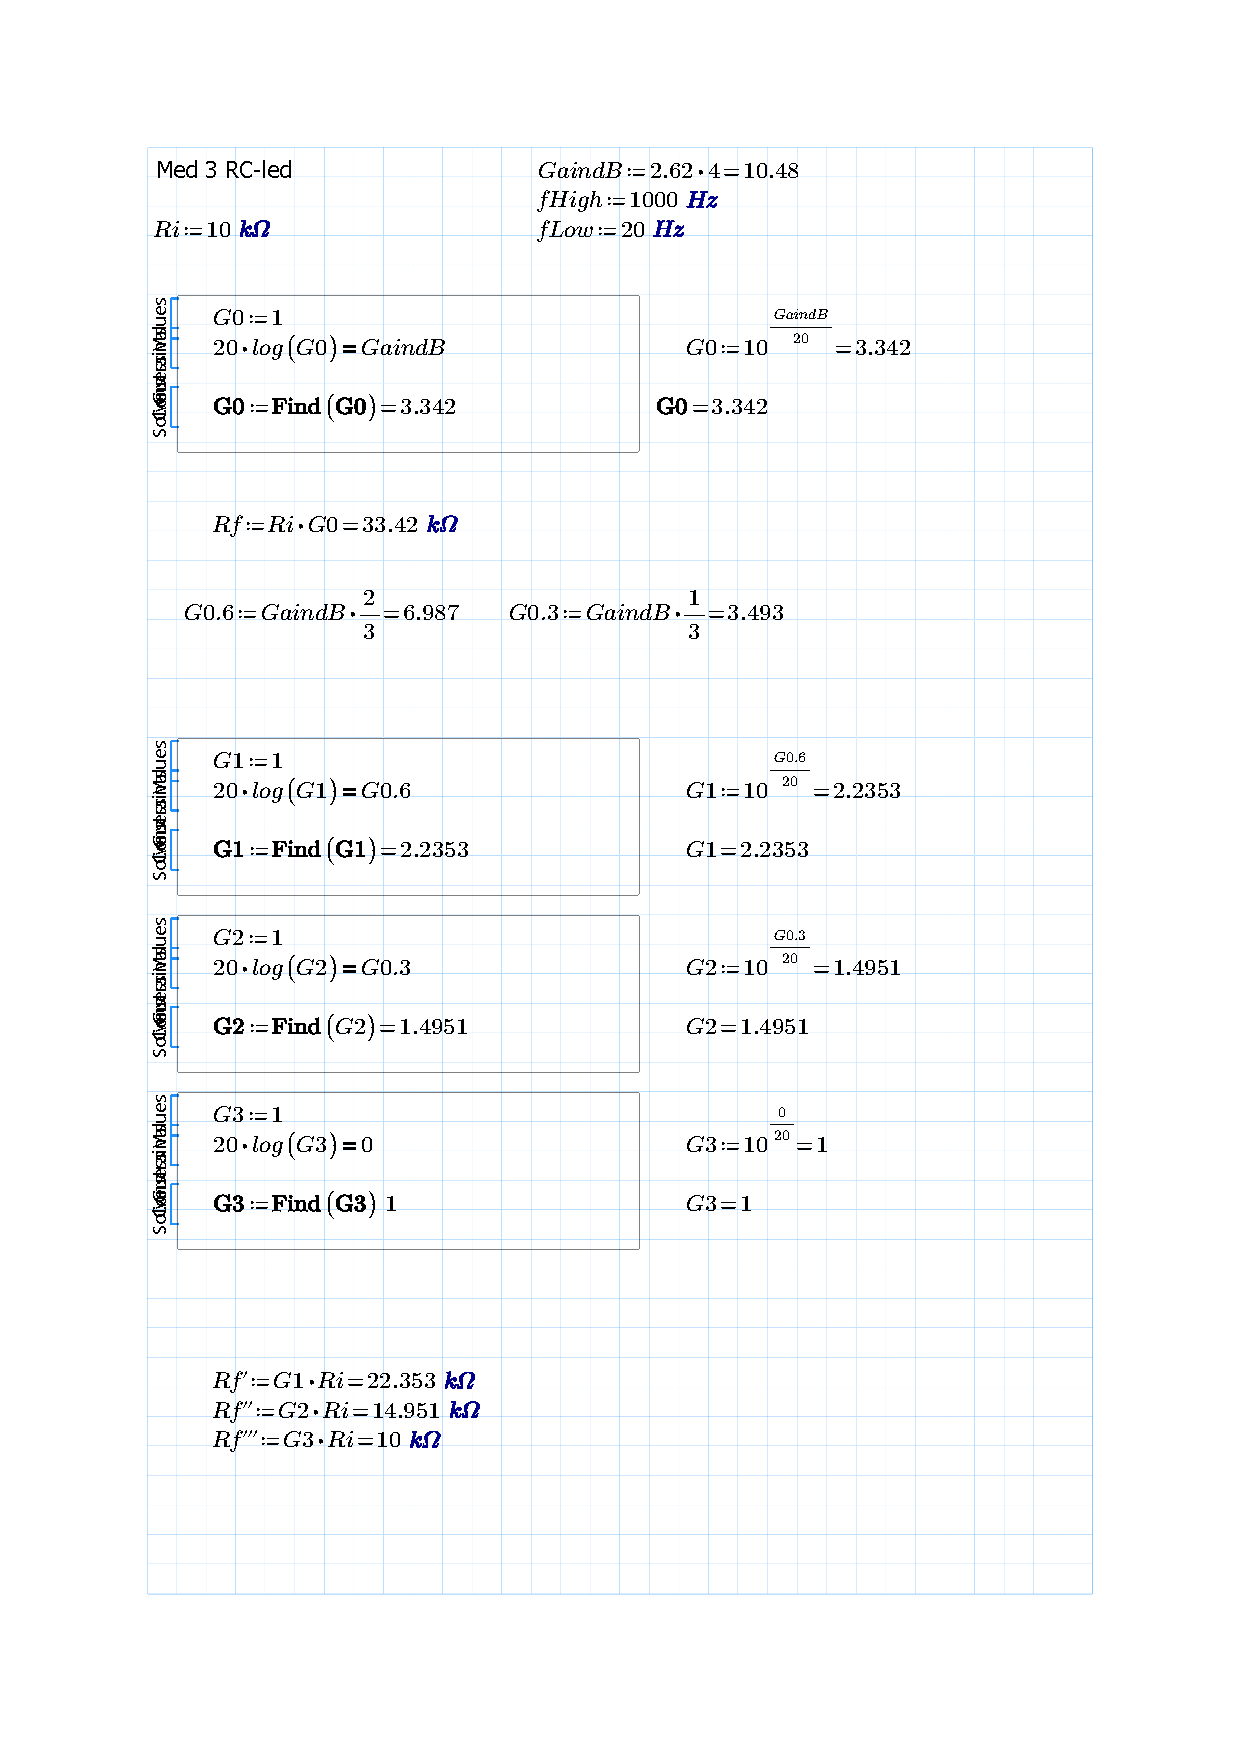
\includepdf[pages={-}]{Content/Bilag/3RCledGain10_48.pdf}
%
\chapter{Beregninger for 20.96 dB forstærkning}
Indeholder beregninger for filtre som giver 20.96 dB forstærkning.
\label{app:3RCledGain20.96}
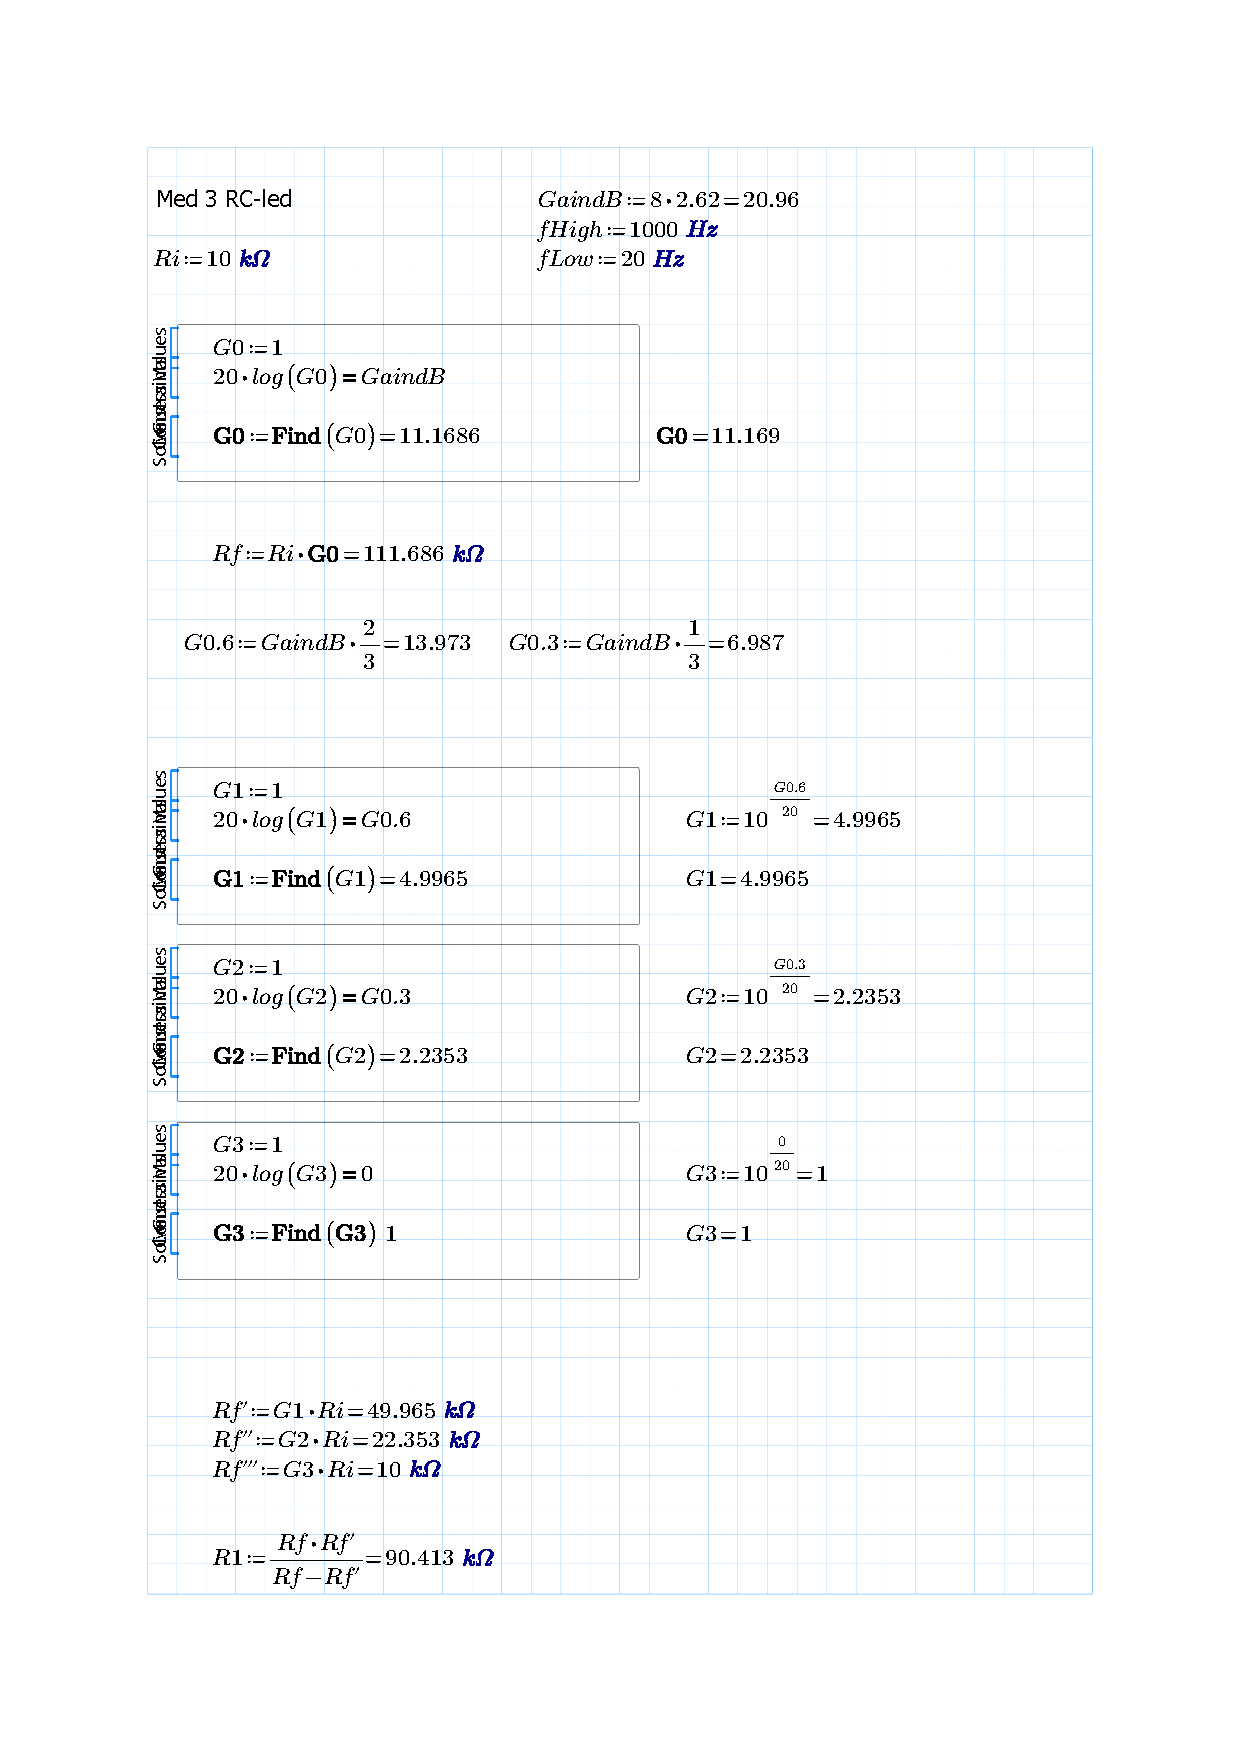
\includepdf[pages={-}]{Content/Bilag/3RCledGain20_96.pdf}
%
%\chapter{Beregning af RC-led}
\label{app:BeregningAfRCLed}
 %  ______ _     _          _ 
 % |  ____| |   | |        | |
 % | |__  | |_  | | ___  __| |
 % |  __| | __| | |/ _ \/ _` |
 % | |____| |_  | |  __/ (_| |
 % |______|\__| |_|\___|\__,_|
\subsection{1 RC-led}
Når vi regner med et RC-led, skal vi sikre at vi får en forstærkning på 1, svarende til 0dB. 
%
\begin{equation}
	G_1 = 1 = \frac{10K\Omega}{10K\Omega}
\end{equation}
\noindent
%
Så finder vi tilbagekoblingsmodstanden ved $G_{1}$
%
\begin{equation}
	R_f' = R_i*G_1 = 10K\Omega*1 = 10K\Omega
\end{equation}
\noindent
%
Så kan vi beregne $R_{1}$
%
\begin{equation}
	R_1 = \frac{R_f*R_f'}{R_f-R_f'} = \frac{13.335K\Omega*10K\Omega}{13.335K\Omega-10K\Omega} = 39.983K\Omega
\end{equation}
\noindent
 %  _______      _          _ 
 % |__   __|    | |        | |
 %    | | ___   | | ___  __| |
 %    | |/ _ \  | |/ _ \/ _` |
 %    | | (_) | | |  __/ (_| |
 %    |_|\___/  |_|\___|\__,_|
\subsection{2 RC-led}
%
Når vi regner med to RC-led, så skal vi sikre at forstærkningen $G_{0}$ fordeles ligeligt mellem de to led, 
%
\begin{equation}
	G_0 = 2.5dB
\end{equation}
\noindent
%
Så kan vores forstærkning i db omregnes til almindelig tal
%
\begin{equation}
	G_0 = 10^{\frac{2.5}{20}} = 1.3335
\end{equation}
\noindent
%
Fordelingen af forstærkning regnes i dB
%
\begin{equation}
	G_1 = 2.5dB*\frac{1}{2} = 1.25dB
\end{equation}
\noindent
%
Så regner vi forstærkningen om fra dB til almindelige tal
%
\begin{equation}
	G_1 = 10^{\frac{1.25}{20}} = 1.1548
\end{equation}
\noindent
%
Så regner forstærkningen for det næste led, som skal gå mod 0
%
\begin{equation}
	G_2 = 2.5dB*0 = 0dB
\end{equation}
\noindent
%
Vores forstærkning kan så omregnes fra dB til almindelige tal
%
\begin{equation}
	G_2 = 10^{\frac{0}{20}} = 1
\end{equation}
\noindent
%
Resultatet angiver hvor meget hvert af de to RC-led skal forstærke. Det er nu muligt at beregne tilbagekoblingsmodstanden for det første led
%
\begin{equation}
	R_f' = R_i*G_1 = 10K\Omega*1.1548 = 11.548K\Omega
\end{equation}
\noindent
%
Så kan vi beregne tilbagekoblingsmodstanden for det andet led
%
\begin{equation}
	R_f'' = R_i*G_2 = 10K\Omega*1 = 10K\Omega
\end{equation}
\noindent
%
Så kan vi regne $R_{1}$
%
\begin{equation}
	R_1 = \frac{R_f*R_f'}{R_f-R_f'} = \frac{13.335K\Omega*11.548K\Omega}{13.335K\Omega-11.548K\Omega} = 86.155K\Omega
\end{equation}
\noindent
%
Så kan vi regne $R_{2}$
%
\begin{equation}
	R_2 = \frac{R_f'*R_f''}{R_f'-R_f''} = \frac{11.548K\Omega*10K\Omega}{11.548K\Omega-10K\Omega} = 74.607K\Omega
\end{equation}
\noindent
 %  _______         _          _ 
 % |__   __|       | |        | |
 %    | |_ __ ___  | | ___  __| |
 %    | | '__/ _ \ | |/ _ \/ _` |
 %    | | | |  __/ | |  __/ (_| |
 %    |_|_|  \___| |_|\___|\__,_|
\subsection{3 RC-led}
%
Når vi regner med tre RC-led, så skal vi sikre at forstærkningen $G_{0}$ fordeles ligeligt mellem de tre led, 
%
\begin{equation}
	G_0 = 2.5dB
\end{equation}
\noindent
%
Så kan vores forstærkning i db omregnes til almindelig tal
%
\begin{equation}
	G_0 = 10^{\frac{2.5}{20}} = 1.3335
\end{equation}
\noindent
%
Fordelingen af forstærkning regnes i dB
%
\begin{equation}
	G_1 = 2.5dB*\frac{2}{3} = 1.667dB
\end{equation}
\noindent
%
Så regner vi forstærkningen om fra dB til almindelige tal
%
\begin{equation}
	G_1 = 10^{\frac{1.667}{20}} = 1.2115
\end{equation}
\noindent
%
Så regner vi forstærkningen for det næste led
%
\begin{equation}
	G_2 = 2.5dB*\frac{1}{3} = 0.833dB
\end{equation}
\noindent
%
Vores forstærkning kan så omregnes fra dB til almindelige tal
%
\begin{equation}
	G_2 = 10^{\frac{0.833}{20}} = 1.1007
\end{equation}
\noindent
%
Så regner vi forstærkningen fra det tredje led mod 0
%
\begin{equation}
	G_3 = 2.5dB*0 = 0dB
\end{equation}
\noindent
%
Vores forstærkning kan så omregnes fra dB til almindelige tal
%
\begin{equation}
	G_3 = 10^{\frac{0}{20}} = 1
\end{equation}
\noindent
%
Det er nu muligt at beregne tilbagekoblingsmodstanden for det første led
%
\begin{equation}
	R_f' = R_i*G_1 = 10K\Omega*1.212 = 12.115K\Omega
\end{equation}
\noindent
%
Så kan vi beregne tilbagekoblingsmodstanden for det andet led
%
\begin{equation}
	R_f'' = R_i*G_2 = 10K\Omega*1.1007 = 11.007K\Omega
\end{equation}
\noindent
%
Så kan vi beregne tilbagekoblingsmodstanden for det sidste led
%
\begin{equation}
	R_f''' = R_i*G_3 = 10K\Omega*1 = 10K\Omega
\end{equation}
\noindent
%
Så kan vi regne $R_{1}$
%
\begin{equation}
	R_1 = \frac{R_f*R_f'}{R_f-R_f'} = \frac{13.335K\Omega*12.115K\Omega}{13.335K\Omega-12.115K\Omega} = 132.433K\Omega
\end{equation}
\noindent
%
Så kan vi regne $R_{2}$
%
\begin{equation}
	R_2 = \frac{R_f'*R_f''}{R_f'-R_f''} = \frac{12.115K\Omega*11.007K\Omega}{12.115K\Omega-11.007K\Omega} = 120.318K\Omega
\end{equation}
%
Så kan vi regne $R_{3}$
%
\begin{equation}
	R_3 = \frac{R_f''*R_f'''}{R_f''-R_f'''} = \frac{11.007K\Omega*10K\Omega}{11.007K\Omega-10K\Omega} = 109.311K\Omega
\end{equation}
 %  ______ _            _          _ 
 % |  ____(_)          | |        | |
 % | |__   _ _ __ ___  | | ___  __| |
 % |  __| | | '__/ _ \ | |/ _ \/ _` |
 % | |    | | | |  __/ | |  __/ (_| |
 % |_|    |_|_|  \___| |_|\___|\__,_|
\subsection{4 RC-led}
%
Når vi regner med fire RC-led, så skal vi sikre at forstærkningen $G_{0}$ fordeles ligeligt mellem de fire led, 
%
\begin{equation}
	G_0 = 2.5dB
\end{equation}
\noindent
%
Så kan vores forstærkning i db omregnes til almindelig tal
%
\begin{equation}
	G_0 = 10^{\frac{2.5}{20}} = 1.3335
\end{equation}
\noindent
%
Fordelingen af forstærkning regnes i dB
%
\begin{equation}
	G_1 = 2.5dB*\frac{3}{4} = 1.875dB
\end{equation}
\noindent
%
Så regner vi forstærkningen om fra dB til almindelige tal
%
\begin{equation}
	G_1 = 10^{\frac{1.875}{20}} = 1.2409
\end{equation}
\noindent
%
Så regner vi forstærkningen for det næste led
%
\begin{equation}
	G_2 = 2.5dB*\frac{2}{4} = 1.250dB
\end{equation}
\noindent
%
Vores forstærkning kan så omregnes fra dB til almindelige tal
%
\begin{equation}
	G_2 = 10^{\frac{1.250}{20}} = 1.1548
\end{equation}
\noindent
%
Så regner vi forstærkningen fra det tredje led 
%
\begin{equation}
	G_3 = 2.5dB*\frac{1}{4} = 0.625dB
\end{equation}
\noindent
%
Vores forstærkning kan så omregnes fra dB til almindelige tal
%
\begin{equation}
	G_3 = 10^{\frac{0.625}{20}} = 1.0746
\end{equation}
\noindent
%
Så regner vi forstærkningen fra det fjerde led, mod 0 
%
\begin{equation}
	G_4 = 2.5dB*0 = 0dB
\end{equation}
\noindent
%
Vores forstærkning kan så omregnes fra dB til almindelige tal
%
\begin{equation}
	G_4 = 10^{\frac{0}{20}} = 1
\end{equation}
\noindent
%
Det er nu muligt at beregne tilbagekoblingsmodstanden for det første led
%
\begin{equation}
	R_f' = R_i*G_1 = 10K\Omega*1.2409 = 12.409K\Omega
\end{equation}
\noindent
%
Så kan vi beregne tilbagekoblingsmodstanden for det andet led
%
\begin{equation}
	R_f'' = R_i*G_2 = 10K\Omega*1.1548 = 11.548K\Omega
\end{equation}
\noindent
%
Så kan vi beregne tilbagekoblingsmodstanden for det tredje led
%
\begin{equation}
	R_f''' = R_i*G_3 = 10K\Omega*1.0746 = 10.746K\Omega
\end{equation}
\noindent
%
Så kan vi beregne tilbagekoblingsmodstanden for det sidste led
%
\begin{equation}
	R_f'''' = R_i*G_4 = 10K\Omega*1 = 10K\Omega
\end{equation}
\noindent
%
Så kan vi regne $R_{1}$
%
\begin{equation}
	R_1 = \frac{R_f*R_f'}{R_f-R_f'} = \frac{13.335K\Omega*12.409K\Omega}{13.335K\Omega-12.409K\Omega} = 178.737K\Omega
\end{equation}
\noindent
%
Så kan vi regne $R_{2}$
%
\begin{equation}
	R_2 = \frac{R_f'*R_f''}{R_f'-R_f''} = \frac{12.409K\Omega*11.548K\Omega}{12.409K\Omega-11.548K\Omega} = 166.328K\Omega
\end{equation}
%
Så kan vi regne $R_{3}$
%
\begin{equation}
	R_3 = \frac{R_f''*R_f'''}{R_f''-R_f'''} = \frac{11.548K\Omega*10.746K\Omega}{11.548K\Omega-10.746K\Omega} = 154.780K\Omega
\end{equation}
%
Så kan vi regne $R_{4}$
%
\begin{equation}
	R_4 = \frac{R_f'''*R_f''''}{R_f'''-R_f''''} = \frac{10.746K\Omega*10K\Omega}{10.746K\Omega-10K\Omega} = 144.034K\Omega
\end{equation}
 %  ______               _          _ 
 % |  ____|             | |        | |
 % | |__ ___ _ __ ___   | | ___  __| |
 % |  __/ _ \ '_ ` _ \  | |/ _ \/ _` |
 % | | |  __/ | | | | | | |  __/ (_| |
 % |_|  \___|_| |_| |_| |_|\___|\__,_|
 \subsection{5 RC-led}
%
Når vi regner med fire RC-led, så skal vi sikre at forstærkningen $G_{0}$ fordeles ligeligt mellem de fire led, 
%
\begin{equation}
	G_0 = 2.5dB
\end{equation}
\noindent
%
Så kan vores forstærkning i db omregnes til almindelig tal
%
\begin{equation}
	G_0 = 10^{\frac{2.5}{20}} = 1.3335
\end{equation}
\noindent
%
Fordelingen af forstærkning regnes i dB
%
\begin{equation}
	G_1 = 2.5dB*\frac{4}{5} = 2dB
\end{equation}
\noindent
%
Så regner vi forstærkningen om fra dB til almindelige tal
%
\begin{equation}
	G_1 = 10^{\frac{2}{20}} = 1.2589
\end{equation}
\noindent
%
Så regner vi forstærkningen for det næste led
%
\begin{equation}
	G_2 = 2.5dB*\frac{3}{5} = 1.5dB
\end{equation}
\noindent
%
Vores forstærkning kan så omregnes fra dB til almindelige tal
%
\begin{equation}
	G_2 = 10^{\frac{1.5}{20}} = 1.1885
\end{equation}
\noindent
%
Så regner vi forstærkningen fra det tredje led 
%
\begin{equation}
	G_3 = 2.5dB*\frac{2}{5} = 1dB
\end{equation}
\noindent
%
Vores forstærkning kan så omregnes fra dB til almindelige tal
%
\begin{equation}
	G_3 = 10^{\frac{1}{20}} = 1.122
\end{equation}
\noindent
%
Så regner vi forstærkningen fra det fjerde led, mod 0 
%
\begin{equation}
	G_4 = 2.5dB*0 = 0.5dB
\end{equation}
\noindent
%
Vores forstærkning kan så omregnes fra dB til almindelige tal
%
\begin{equation}
	G_4 = 10^{\frac{0.5}{20}} = 1.059
\end{equation}
\noindent
%
Så regner vi forstærkningen fra det femte led, mod 0 
%
\begin{equation}
	G_4 = 2.5dB*0 = 0dB
\end{equation}
\noindent
%
Vores forstærkning kan så omregnes fra dB til almindelige tal
%
\begin{equation}
	G_5 = 10^{\frac{0}{20}} = 1
\end{equation}
\noindent
%
Det er nu muligt at beregne tilbagekoblingsmodstanden for det første led
%
\begin{equation}
	R_f' = R_i*G_1 = 10K\Omega*1.2409 = 12.589K\Omega
\end{equation}
\noindent
%
Så kan vi beregne tilbagekoblingsmodstanden for det andet led
%
\begin{equation}
	R_f'' = R_i*G_2 = 10K\Omega*1.1548 = 11.885K\Omega
\end{equation}
\noindent
%
Så kan vi beregne tilbagekoblingsmodstanden for det tredje led
%
\begin{equation}
	R_f''' = R_i*G_3 = 10K\Omega*1.0746 = 11.22K\Omega
\end{equation}
\noindent
%
Så kan vi beregne tilbagekoblingsmodstanden for det fjerde led
%
\begin{equation}
	R_f'''' = R_i*G_4 = 10K\Omega*1 = 10.593K\Omega
\end{equation}
\noindent
%
%
Så kan vi beregne tilbagekoblingsmodstanden for det sidste led
%
\begin{equation}
	R_f''''' = R_i*G_5 = 10K\Omega*1 = 10K\Omega
\end{equation}
\noindent
%
Så kan vi regne $R_{1}$
%
\begin{equation}
	R_1 = \frac{R_f*R_f'}{R_f-R_f'} = \frac{13.335K\Omega*12.589K\Omega}{13.335K\Omega-12.589K\Omega} = 225.053K\Omega
\end{equation}
\noindent
%
Så kan vi regne $R_{2}$
%
\begin{equation}
	R_2 = \frac{R_f'*R_f''}{R_f'-R_f''} = \frac{12.589K\Omega*11.885K\Omega}{12.589K\Omega-11.885K\Omega} = 212.464K\Omega
\end{equation}
%
Så kan vi regne $R_{3}$
%
\begin{equation}
	R_3 = \frac{R_f''*R_f'''}{R_f''-R_f'''} = \frac{11.885K\Omega*11.22K\Omega}{11.885K\Omega-11.22K\Omega} = 200.578K\Omega
\end{equation}
%
Så kan vi regne $R_{4}$
%
\begin{equation}
	R_4 = \frac{R_f'''*R_f''''}{R_f'''-R_f''''} = \frac{11.22K\Omega*10.593K\Omega}{11.22K\Omega-10.593K\Omega} = 189.358K\Omega
\end{equation}
%
Så kan vi regne $R_{5}$
%
\begin{equation}
	R_5 = \frac{R_f''''*R_f'''''}{R_f''''-R_f'''''} = \frac{10.593K\Omega*10K\Omega}{10.593K\Omega-10K\Omega} = 178.766K\Omega
\end{equation}
%\chapter{Formelsamling}
\label{Formelsamling}
%
\begin{tabularx}{\textwidth}{ |X|X| }
%  \hline
%  \multicolumn{1}{ |c|l| }{Team sheet} & TEST TESTTEST\\
  \hline
  \bigskip
  \(\displaystyle 	 L_p=\left(\frac{10}{\alpha_f} * lg A_f\right) dB - L_U + 94dB \) 
  & 
  Formel til udregning af, hvilket lydtryksniveau en ren tone skal afspilles ved, for at den perciperes som værende lige så høj som referencetonen ved en given phon-kurve.
  
  \bigskip
  $f$ = Frekvens givet i hertz
  
  \noindent
  $L_P$ = Lydtryksniveauet givet i dB
  
  \noindent 
  $L_U$ = Størrelsen af den lineære overføringsfunktion, normaliseret ved 1000Hz
  
  \bigskip
  Formelen gør sig kun gældende fra 20phon til 90phon, med forbehold for at 90phon er begrænset til frekvenserne mellem 20Hz og 4000Hz og 80phon er begrænset til frekvenser mellem 5000Hz til 12500Hz. Uden for denne afgrænsning vil formlen kun fungere informativt. \\
  \hline 
  \bigskip
  \(\displaystyle A_f = 4.47 * 10^{-3} * \left(10^{0.025*L_N} - 1.15\right) + \left[0.4*10^{\left(\frac{T_f + L_U}{10} - 9\right)}\right]^{\alpha_f}\) 
  &
  Variablen $A_f$ beskriver sammenhængen mellem \textit{Loudness-Level} og grænseværdien for menneskets hørelse i forhold til en valgt frekvens, samt menneskets evne til at percipere en tone ved frekvensen.
  
  \bigskip
  $L_N$ = \textit{Loudness-Level} givet i phon
  
  \noindent
  $T_f$ = Høretærsklen
  
  \noindent
  $\alpha_f$ = Eksponenten for perception af \textit{Loudness}
  
  \bigskip
  Værdierne for $A_f$ og $\alpha_f$ er de samme i de to formler. \\
  \hline
   \bigskip
  \(\displaystyle datapunkt = (phon_{ref}-phon_{level})-
  (dB_{ref}-dB_{level})\) 
  &
  Formel til at udregne et nyt datapunkt bestående af differencen mellem referencen og en specifik phon-kurve ved en bestemt frekvens. Differencen mellem $phon_{ref}$ og $phon_{level}$ angiver forskydningsfaktoren. 
  
  \bigskip
  $phon_{ref}$ = Referencen på 80phon
  
  \noindent
  $phon_{level}$ = Den specifikke phon-kurve, hvorfra differencen skal findes
  
  \noindent
  $dB_{ref}$ = Referencens lydtryksniveau målt ved den pågældende frekvens
  
  \noindent
  $dB_{level}$ = Den specifikke phon-kurves lydtryksniveau målt ved den pågældende frekvens \\
  \hline
\end{tabularx}


\begin{tabularx}{\textwidth}{ |X|X| }
%  \hline
%  \multicolumn{1}{ |c|l| }{Team sheet} & TEST TESTTEST\\
  \hline
  \bigskip
  \(\displaystyle \Delta L = 10*log\left[\frac{(I+\Delta I)}{I}\right]\) 
  &
  \textit{Webers Fraction} er en formel til udregning af JND i forhold til detektering af intensitetsforskelle (lydtryksniveauer) vedrørende \textit{Loudness}. Formlen gør sig gældende når JND skal angives i dB.
  
  \bigskip
  $\Delta L$ = JND for den hørbare ændring i \textit{Loudness}
  
  \noindent 
  $\Delta I$ = Den mindste perciperede ændring i intensitet (lydtryksniveau)
  
  \noindent
  $I$ = Tonens intensitet (lydtryksniveau)
  \noindent
    
  \bigskip
  Forholdet mellem $\Delta I$ og $I$ antages forværende konstant. For \textit{Wideband Noise} er JND mellem 0.5dB og 1dB for lydtryksniveauer mellem 20dB og 100dB. Formlen gør sig ikke gældende for rene toner.\\
  \hline
\end{tabularx}



%